% This file was created with tikzplotlib v0.10.1.
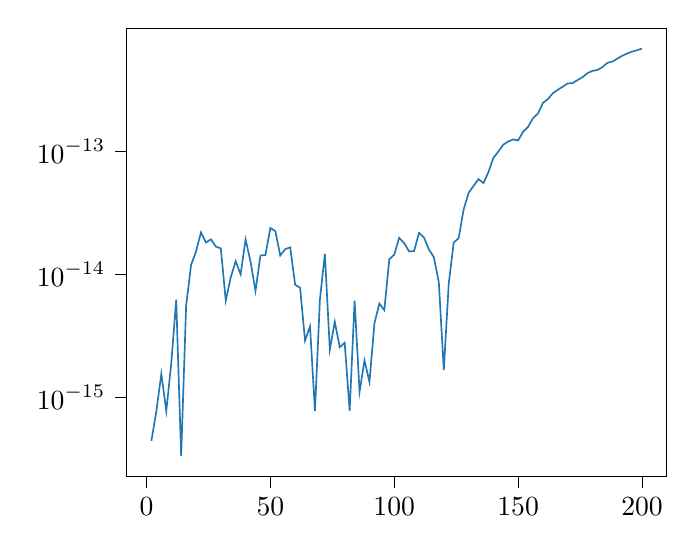
\begin{tikzpicture}

\definecolor{darkgray176}{RGB}{176,176,176}
\definecolor{steelblue31119180}{RGB}{31,119,180}

\begin{axis}[
log basis y={10},
tick align=outside,
tick pos=left,
x grid style={darkgray176},
xmin=-7.9, xmax=209.9,
xtick style={color=black},
y grid style={darkgray176},
ymin=2.27534484038668e-16, ymax=9.94758428519327e-13,
ymode=log,
ytick style={color=black},
ytick={1e-17,1e-16,1e-15,1e-14,1e-13,1e-12,1e-11},
yticklabels={
  \(\displaystyle {10^{-17}}\),
  \(\displaystyle {10^{-16}}\),
  \(\displaystyle {10^{-15}}\),
  \(\displaystyle {10^{-14}}\),
  \(\displaystyle {10^{-13}}\),
  \(\displaystyle {10^{-12}}\),
  \(\displaystyle {10^{-11}}\)
}
]
\addplot [semithick, steelblue31119180]
table {%
2 4.44091274492872e-16
4 7.77156276056287e-16
6 1.55431223447522e-15
8 7.77157017210116e-16
10 1.88737956537924e-15
12 6.21724893790088e-15
14 3.33067489722698e-16
16 5.55111512312578e-15
18 1.18793863634892e-14
20 1.53210777398272e-14
22 2.18713935851156e-14
24 1.80966353013901e-14
26 1.92068583260152e-14
28 1.67643676718399e-14
30 1.62092561595273e-14
32 6.10622663543836e-15
34 9.43689570931383e-15
36 1.27675647831893e-14
38 9.99200722162641e-15
40 1.92068583260152e-14
42 1.26565424807268e-14
44 7.32747196252603e-15
46 1.4210854715202e-14
48 1.43218770176645e-14
50 2.37587727269783e-14
52 2.24265050974282e-14
54 1.4210854715202e-14
56 1.59872115546023e-14
58 1.65423230669148e-14
60 8.21565038222616e-15
62 7.7715611723761e-15
64 2.88658028754188e-15
66 3.77475828372553e-15
68 7.77156223116728e-16
70 6.21724893790088e-15
72 1.46549439250521e-14
74 2.44249107769182e-15
76 4.10782519111308e-15
78 2.5535131683961e-15
80 2.77555756156289e-15
82 7.77156805451879e-16
84 6.10622663543836e-15
86 1.11022334226251e-15
88 1.99840165608352e-15
90 1.33226762955019e-15
92 3.99680288865056e-15
94 5.77316015156729e-15
96 5.10702591327572e-15
98 1.32116539930394e-14
100 1.4432899320127e-14
102 1.97619698383278e-14
104 1.7874590696465e-14
106 1.53210777398272e-14
108 1.54321000422897e-14
110 2.16493489801906e-14
112 1.98729921407903e-14
114 1.58761892521397e-14
116 1.37667655053519e-14
118 8.54871728961371e-15
120 1.66533464281685e-15
122 8.43769498715119e-15
124 1.80966353013901e-14
126 1.96509475358653e-14
128 3.35287353436797e-14
130 4.57411886145564e-14
132 5.21804821573824e-14
134 5.91748872125208e-14
136 5.49560397189452e-14
138 6.7390537594747e-14
140 8.79296635503124e-14
142 9.9031893796564e-14
144 1.12798659301916e-13
146 1.19682042054592e-13
148 1.24344978758018e-13
150 1.22013510406305e-13
152 1.43662859386495e-13
154 1.57429624891847e-13
156 1.85074178205014e-13
158 2.01838545876853e-13
160 2.4624746686186e-13
162 2.6434410216325e-13
164 2.94875235340442e-13
166 3.14970272086157e-13
168 3.33399974294935e-13
170 3.54272167157887e-13
172 3.56714657812063e-13
174 3.77586850675016e-13
176 3.98570065840431e-13
178 4.30100399739786e-13
180 4.48419079646101e-13
182 4.55746551608627e-13
184 4.8061554736023e-13
186 5.20805620851661e-13
188 5.33018074122538e-13
190 5.63216140392342e-13
192 5.94302385081846e-13
194 6.21280804580238e-13
196 6.43152198165353e-13
198 6.59916565837193e-13
200 6.79567513373058e-13
};
\end{axis}

\end{tikzpicture}
